\appendices

\section{Explanation of Expected QoI with Random Image Selection}
\label{sec:expl_exp_qoi}

\subsection{Top-K}
First, we explain the expected number of images that are from the same set as the target image in the Top-K algorithm when images are selected from the entire image pool at random.  We define the following:  

\begin{itemize}
	\item $n$ = total number of images (summed over all sets)
	\item $S$ = number of sets
	\item $S_k$ = set of target image
	\item $k$ = number of images selected
	\item $N_{S}$ = number of images in each set (for simplicity, assumed to be the same for all sets)
	\item $x$ = number of images returned from set $S_k$
\end{itemize}

\begin{equation}
	P( X = x | k ) = \left\{ \,
	\begin{IEEEeqnarraybox}[][c]{l?s}
		\IEEEstrut
		\frac{{k \choose x} * {n-k \choose k-x} }{ {n \choose k}} & if $k \leq N_S$, \\
		\frac{ {N_{S} \choose x} * {n-N_{S} \choose k-x}}{{n \choose k}} & if $N_S < k \leq n-N_S$
		\IEEEstrut
	\end{IEEEeqnarraybox}
	\right.
\label{eq:prob_topk_rand}
\end{equation}
 
%If $k \leq N_{S}$, then 
%\begin{equation}
%	p(X = x | k) = \frac{{k \choose x} * {n-k \choose k-x} }{ {n \choose k}}, \forall x \leq k
%\end{equation}
%Otherwise, $p(X = x | k) = 0$.
Equation \ref{eq:prob_topk_rand} provides the probability that $x$ of the $k$ selected images will be from the target set.  When $k \leq N_S$, the total number of possible combinations of choosing $x$ from the target set and $k-x$ from the $n - N_{S_k}$ remaining images over the entire sample space ($n$ choose $k$).  
%Naturally, we cannot end up with more images from the target set than the number of images selected, and, thus the probability of $x > k$ is zero.  
When $N_{S} < k < n-N_{S}$, then we consider the possible combinations of choosing $x$ images from the target set and $k-x$ images from the remaining $n-N_{S}$ images.
This probability formula can then be used to derive the expected values of $x$ displayed in Figure \ref{fig:topkAvgNumSameSet}. 
%Finally, when $k > n-N_{S}$, then $k - (n-N_{S} + x)$ images must be from the target set by the pigeonhole principle, so the $p(X = x) = 0$ for all $k > n - N_{S} + x$.  Otherwise, the same expression as directly above is true.

%\begin{equation}
%	p(X = x | N_S < k < n - N_S) = \frac{ {N_{S} \choose x} * {n-N_{S} \choose k-x}}{{n \choose k}}
%\end{equation}

\subsection{Clustering}
For Clustering, we want to determine the probability that we will cover each of the $S$ sets with at least one of the $k$ chosen images if we had chosen them randomly.  We will call $X_i$ the random variable that represents the number of images from set $i$ in the results.  We use the following expression:

\begin{equation}
	P( X_i > 0 , \forall i | k) = (1 - P(X_i = 0))^{S}
\end{equation}
where $X_i$ is given by a multivariate hypergeometric distribution, which gives us the following:
\begin{equation}
	P(X_i = 0 | k) = \frac{{n-N_s \choose k}}{{n \choose k}}
\end{equation}

This probability expression is plotted directly against the percentage of trials in which all sets were covered in experiments using the Clustering algorithm in Figure \ref{fig:clusterAvgNumSetsCov}.


\section{Derivation of Traffic Factor for Example Topologies}
\label{sec:derivation_TFs}

With a goal of determining maximum scalability and QoI-satisfiability limits, we focus on the bottleneck node, $b$, which is the node that results in the largest mean $\mu_{TF_x}$ value. For topologies with regular patterns like the line and grid networks, finding the bottleneck node and expressions to capture the expected traffic through it is intuitive. When handling non-uniform topologies, we use some straightforward processing on the graph to determine the bottleneck and appropriate values for the traffic factor.

\subsection{Clique Network Traffic Factor}
In a clique network, all nodes have a direct link to every other node, so no node is required to forward other nodes' traffic.  Therefore, we can simply set $\mu_{TF} = 1$ and $\sigma_{TF} = 0$.

\subsection{Line Network Traffic Factor}

For a line network, first, let us look at the number of paths that go through the bottleneck node, which is the center node for a line network.  We will assume that $N$ is odd here, for simplicity of notation, but the logic is the same for even values of $N$.  Since there are $\frac{N-1}{2}$ nodes on each side the center node, the total number of paths that go through it is
\begin{equation*}
%	\rho(\frac{N}{2}) = 2(\frac{N}{2}-1)^2
%	\rho(b) = 2(\frac{N}{2}-1)^2
	\rho(b) = 2(\frac{N-1}{2})^2
\end{equation*}

Then, since there are $N$ flows and $N*(N-1)$ total paths in the network, we can approximate the probability of each path containing a flow as $p_f = \frac{1}{N-1}$.  Then, $TF_x$ will be a Binomial random variable with $n=\rho(b)$ and $p=\frac{1}{N-1}$.  Therefore, $p$ approaches zero as the network size, $N$, and thus, $n$, increases, so we use a Poisson approximation for $TF_b$, giving the following distribution:  
%We note that in other traffic patterns, e.g., when $p$ does not approach $1$ or $0$, a normal approximation may be used instead.   
\begin{equation*}
	f_{TF_b}(t) = e^{-(\frac{N-1}{2})}\frac{(\frac{N-1}{2})^{t}}{t!}
\end{equation*} 

\subsection{Grid Network Traffic Factor}

Again, the bottleneck node, i.e., the node with the highest number of paths going through it is the center node, and we give the derivation for when $\sqrt{N}$ is odd, but the logic follows similarly for even values.  As proved in \cite{lattice_nets_cap_opt_routing}, the most optimal routing scheme for maximum capacity is ``Row-First, Column-Second" routing, so we assume paths follow this approach.  Again, we adopt a traffic pattern in which each node is the source of exactly one flow and that the destination is uniformly chosen from all other $N-1$ nodes.  
%Node $i$, then, has a $\frac{1}{N-2}$ chance of choosing each non-center node.  
For each source node, we can determine the number of destinations that route through the center.  We separate nodes into two categories for this counting.

\begin{figure}
\begin{centering}
    \includegraphics[scale=0.39]{figures/TF_proof_fig_color.pdf}
    \caption{Sources and destinations used in proving TF for grid networks}
    \label{fig:TF_proof_fig}
\end{centering}
\end{figure}

First, we consider the nodes circled in set $A$ in Figure \ref{fig:TF_proof_fig}, of which there are $\sqrt{N} \cdot \frac{\sqrt{N}-1}{2}$.  Through manual inspection, one can deduce that the only destination nodes in the figure that result in a path that is relayed by the center node are the two bottom nodes in the center column in the figure, marked with blue.  
%The probability of a node in set $A$ choosing one of these destinations is $P_{A} = \frac{\frac{\sqrt{N}-1}{2}}{N-2}$.
%Now, we can count the total number of nodes for which this probability holds.  From the figure, we can quantify the number of circled nodes, but we must also consider the reverse, i.e. imagine the figure rotated vertically, so the total number of nodes falling into set $A$, including the mirror of those circled in the figure, is $N_A = \sqrt{N} \cdot (\sqrt{N}-1)$.
There are $\frac{\sqrt{N}-1}{2}$ of these destination nodes for the nodes in set $A$, so the total number of paths from the nodes in set $A$ is $\sqrt{N} \cdot (\frac{\sqrt{N}-1}{2})^2$.  Now, if we also consider the reverse, i.e. imagine the figure rotated vertically, then we can give the total number of paths from nodes not in the same row as the center node as $2 \cdot \sqrt{N} \cdot (\frac{\sqrt{N}-1}{2})^2$.
%Now, we can count the total number of nodes for which this probability holds.  From the figure, we can quantify the number of circled nodes, but we must also consider the reverse, i.e. imagine the figure rotated vertically, so the total number of nodes falling into set $A$, including the mirror of those circled in the figure, is $N_A = \sqrt{N} \cdot (\sqrt{N}-1)$.
%Then, the contribution to the TF by nodes in set $A$ is simply the product of $P_A$ and $N_A$:
%\begin{equation}
%	E[TF_{A}] = \frac{\frac{\sqrt{N}-1}{2}}{N-2}  \cdot  \sqrt{N} \cdot (\sqrt{N}-1)
%\end{equation}

Next, we consider the nodes in the same row as the center node, which we call set $B$.  
Here, all destinations on the ``opposite" side of the center as well as those in the same column of the center require being routed through the center node when originating from any nodes in set $B$.  Just as above, we can count the number of paths from the nodes in set $B$ that route through the center and double it to count the reverse.  The resulting number of paths is $2 \cdot (\sqrt{N} \cdot \frac{\sqrt{N}+1}{2}-1) \cdot (\frac{\sqrt{N}-1}{2})$.
%Just as above, we can relate the probability of choosing one of these destinations as $P_{B} = \frac{\frac{\sqrt{N}+1}{2} \cdot \sqrt{N} - 1}{N-2}$ and $N_{B} = \sqrt{N}$, so the expected contribution to TF from set $B$ is
%\begin{equation}
%	E[TF_{B}] = \frac{\frac{\sqrt{N}+1}{2} \cdot \sqrt{N} - 1}{N-2} \cdot 2 \cdot (\frac{\sqrt{N}-1}{2})
%\end{equation}
%
%Since sets $A$ and $B$ account for all non-center nodes in the network, the overall expected traffic factor is just the sum of $E[TF_A]$ and $E[TF_B]$, which simplifies to
%\begin{equation}
%	E[TF] = \frac{\sqrt{N}(N - 2) + 1}{N-2}
%\end{equation}
%which is effectively $\sqrt{N}$ for large $N$.

Adding together these paths and simplifying gives us the following expression for the total number of paths that go through the center node: 
\begin{equation}
%	\rho(\frac{N}{2}) = \sqrt{N} \cdot (N-2) + 1
	\rho(b) = \sqrt{N} \cdot (N-2) + 1
\end{equation}
Just as with line networks, the probability of each path containing a flow is $p_f = \frac{1}{N-1}$, so the traffic factor for the center node of a grid network is approximated with a Poisson distribution:
\begin{equation*}
%	f_{TF_b} = \mathcal{N}( \frac{\sqrt{N} \cdot (N-2) + 1}{N-1}, \frac{\sqrt{N} \cdot (N-2) + 1}{N-1} \cdot ( 1 - \frac{1}{N-1} )  )
	f_{TF_b}(t) = e^{-(\frac{\sqrt{N}\cdot(N-2)+1}{N-1})}\frac{(\frac{\sqrt{N}\cdot(N-2)+1}{N-1})^{t}}{t!}
\end{equation*}
which can be approximated by the following for large values of $N$.  
\begin{equation*}
%	f_{TF_b} = \mathcal{N}( \sqrt{N}, \sqrt{N} \cdot ( 1 - \frac{1}{N-1} )  )
	f_{TF_b}(t) = e^{-(\sqrt{N})}\frac{(\sqrt{N})^{t}}{t!}
\end{equation*}

%Since our goal is to determine the point at which an average flow is no longer sustainable, we derive expressions for $TF$, $CF$, and $DF$ for the network.  In the case of $TF$, we use the value for the node with the largest expected $TF_i$ since flows that are routed through this node are expected to experience that largest delay and are likely to be the first that fail to meet their timeliness requirements.  Values for this example are shown in Table \ref{table:rf_ff_sf_values}. A derivation of $TF$ for a grid network is included in Appendix \ref{sec:grid_tf_proof}.  Details about deriving the other values are explained in \cite{symptotics_journal}.  The equations in Table \ref{table:scal_eqs} can be used to determine QoI and network size limitations.

\subsection{NSF Network}

\begin{figure}
\begin{centering}
    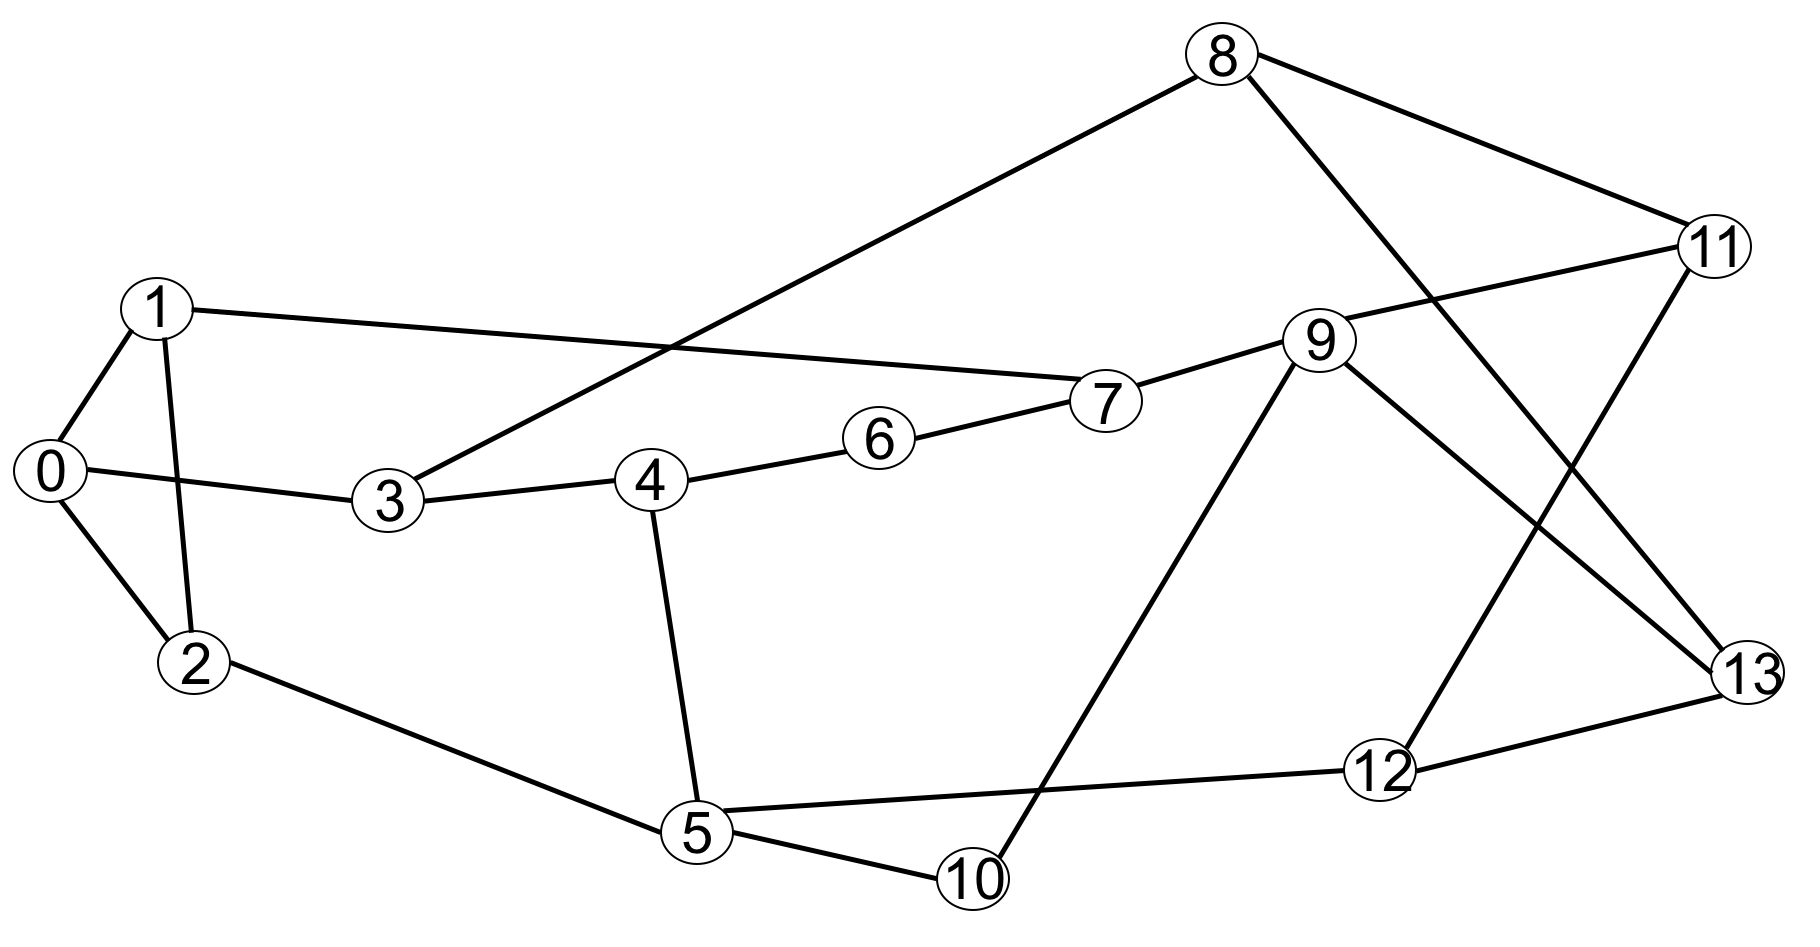
\includegraphics[scale=0.25]{figures/NSF_net.png}
    \caption{Topology of NSFNET network. Node $5$ is on the highest number of shortest paths between all pairs, so it is the bottleneck node.}
    \label{fig:NSF_net}
\end{centering}
\end{figure}

We can also determine the traffic factor for an arbitrary network like the NSFNET topology \cite{nsf_net} shown in Figure \ref{fig:NSF_net}. In cases such as this, the bottleneck may not be immediately evident, but finding it is simply a matter of using any standard shortest path algorithm to find the number of shortest paths on which a node $x$ is present, $\rho(x)$, for all nodes. Then, the bottleneck node is the node with the maximum $\rho()$ value: $b = \argmax_{x} \rho(x)$. In the NSFNET topology, node $5$ is the bottleneck with $\rho(5) = 28$. As above, the probability of each path currently being used to serve a flow is $p_f = \frac{1}{N-1} = \frac{1}{13} = 0.077$. Since this probability is close to zero, the Poisson approximation with parameter $\rho(b)*p_f = 28*0.077 \approx 2.15$ is appropriate for this traffic factor distribution:
\begin{equation*}
  f_{TF_b}(t) = e^{-2.15} \frac{2.15^t}{t!}
\end{equation*}

\section{Proof of Multiplicative Chernoff Bound}
\label{sec:chernoff_bound_proof}

The authors in \cite{mitzenmacher2005probability} prove a different bound for $0 < \eta \leq 1$.  We follow the same logic to prove the following bound for $\eta \geq 1$.

\noindent
{\bf Theorem 1:}
Let $X$ be the sum of independent Poisson trials and $\mu = \mathbb{E}[X]$.  The following bound holds for $\eta \geq 1$:
\begin{equation}
\label{eq:new_chernoff_bound}
	P( TF \geq (1 + \eta)\mu_{TF} ) \leq e^{\frac{-\eta^2}{2+\eta}\mu_{TF}}
\end{equation}

\noindent
{\bf Proof:}
First, we reiterate the following relative Chernoff Bound given in \cite{mitzenmacher2005probability}:  
For any $\eta > 0$, 
\begin{equation}
\label{eq:orig_chernoff_bound}
	P( X \geq (1 + \eta) \mu ) < ( \frac{e^\eta}{(1+\eta)^{(1+\eta)}} )^\mu
\end{equation}
Using (\ref{eq:orig_chernoff_bound}), to prove (\ref{eq:new_chernoff_bound}), we must show that the following holds for $\eta \geq 1$:
\begin{equation}
\label{eq:bound_condition}
	\frac{e^\eta}{(1+\eta)^{(1+\eta)}} \leq e^{\frac{-\eta^2}{2+\eta}}
\end{equation}
Taking the natural logarithm and rearranging, we get
\begin{equation}
	f( \eta ) = \eta - (1+\eta)\ln(1+\eta) + \frac{\eta^2}{2+\eta} \leq 0
\end{equation}
Then, the first and second derivates of $f(\eta)$ with respect to $\eta$ are
\begin{equation}
	f'( \eta ) = -\ln(1+\eta) + \frac{\eta(\eta + 4)}{(\eta+2)^2}
\end{equation}
\begin{equation}
	f''( \eta ) = -\frac{1}{1+\eta} + \frac{8}{(\eta+2)^3}
\end{equation}
Note that $f(1) = -0.053$.  Additionally, for all $\eta \geq 1$, $f'(\eta) < 0$ and $f''(\eta) < 0$.  Therefore, $f(\eta)$ is decreasing and concave down for $\eta \geq 1$.  This fact, along with the fact that $f(1) < 0$, implies that $f(\eta)$ stays negative for $\eta \geq 1$.  Hence, (\ref{eq:bound_condition}) is satisfied, completing our proof.
%Since for $\eta \geq 1$, $f''(\eta)$ is always negative, $f'(\eta)$ is monotonically decreasing in this range.  Realizing that $f'(1) < 0$, then, proves that $f'(\eta)$ is also negative when $\eta \geq 1$.  Therefore, since $f(1) < 0$ also, $f(\eta) < 0$ for all $\eta \geq 1$.
\hfill$\blacksquare$

%\section{Proof of Traffic Factor for Grid Network}
%\label{sec:grid_tf_proof}
%We outline a simple proof for determining the TF of the center node in a grid of $N$ nodes using ``Row-First, Column-Second" routing.  We give the proof for when $\sqrt{N}$ is odd, but the logic follows similarly for even values.
%Assume each node is the source of exactly one flow and that the destination is uniformly chosen from all other $N-1$ nodes.  Node $i$, then, has a $\frac{1}{N-2}$ chance of choosing each non-center node.  
%%For each source node, we can determine the number of destinations that route through the center.  We separate nodes into two categories for this counting.
%
%\begin{figure}
%\begin{centering}
%    \includegraphics[scale=0.32]{figures/TF_proof_fig_color.pdf}
%    \vspace{-4mm}
%    \caption{Sources and destinations used in proving TF for grid networks}
%    \label{fig:TF_proof_fig}
%    \vspace{-6mm}
%\end{centering}
%\end{figure}
%
%First, we consider the nodes circled in set $A$ in Figure \ref{fig:TF_proof_fig}.  
%%Through manual inspection, one can deduce that the only destination nodes in the figure that result in a path that is relayed by the center node are the two bottom nodes in the center column in the figure, marked with blue.  
%The destinations that are relayed through the center are marked in blue in the figure.
%The probability of a node in set $A$ choosing one of these destinations is $P_{A} = \frac{\frac{\sqrt{N}-1}{2}}{N-2}$.
%%Now, we can count the total number of nodes for which this probability holds.  From the figure, we can quantify the number of circled nodes, but we must also consider the reverse, i.e. imagine the figure rotated vertically, so 
%The total number of nodes falling into set $A$, including the mirror of those circled in the figure, is $N_A = \sqrt{N} \cdot (\sqrt{N}-1)$.
%Then, the contribution to the TF by nodes in set $A$ is simply the product of $P_A$ and $N_A$:
%%\begin{equation}
%	$E[TF_{A}] = \frac{\frac{\sqrt{N}-1}{2}}{N-2}  \cdot  \sqrt{N} \cdot (\sqrt{N}-1)$
%%\end{equation}
%
%%Next, we consider the nodes in the same row as the center node, which we call set $B$.  
%%Here, all destinations on the ``opposite" side of the center as well as those in the same column of the center require being routed through the center node when originating from any nodes in set $B$.  Just as above, we can relate the probability of choosing one of these destinations as 
%Similarly, for set $B$: $P_{B} = \frac{\frac{\sqrt{N}+1}{2} \cdot \sqrt{N} - 1}{N-2}$
% and $N_{B} = \frac{\sqrt{N-1}}{2}$, so the expected contribution to TF from set $B$ is
%%\begin{equation}
%	$E[TF_{B}] = \frac{\frac{\sqrt{N}+1}{2} \cdot \sqrt{N} - 1}{N-2} \cdot 2 \cdot (\frac{\sqrt{N}-1}{2})$.
%%\end{equation}
%
%Since sets $A$ and $B$ account for all non-center nodes in the network, the overall expected traffic factor is just the sum of $E[TF_A]$ and $E[TF_B]$, which simplifies to
%\begin{equation}
%	E[TF] = \frac{\sqrt{N}(N - 2) + 1}{N-2}
%\end{equation}
%which is effectively $\sqrt{N}$ for large $N$.
%\vspace{-1.5mm}

